\documentclass[a4paper,12pt]{article}
\usepackage[a4paper,top=1.3cm,bottom=2cm,left=1.5cm,right=1.5cm,marginparwidth=0.75cm]{geometry}
\usepackage{cmap}
\usepackage{mathtext}
\usepackage[T2A]{fontenc}
\usepackage[utf8]{inputenc}
\usepackage[english,russian]{babel}
\usepackage{siunitx}
\usepackage{enumitem}
\usepackage{placeins}

\usepackage{graphicx}
\usepackage{subcaption}
\usepackage{amsmath}

\usepackage{wrapfig}
\usepackage{tabularx}
\usepackage{multirow}

\usepackage{hyperref}
\usepackage[rgb]{xcolor}
\hypersetup{colorlinks=true,urlcolor=blue}
\usepackage{siunitx}
\usepackage{amsmath,amsfonts,amssymb,amsthm,mathtools}
\usepackage{mathtools}
\usepackage{icomma}
\mathtoolsset{showonlyrefs=false}
\usepackage{euscript}
\usepackage{mathrsfs}
\DeclareMathOperator{\sgn}{\mathop{sgn}}
\newcommand*{\hm}[1]{#1\nobreak\discretionary{}
{\hbox{$\mathsurround=0pt #1$}}{}}

%%% Заголовок
\newcommand\labname{Электронный парамагнитный резонанс}
\newcommand\labnumber{5.10.1}


\author{Макаров Лев Евгеньевич}
\title{Лабораторная работа №\labnumber

\labname
}

\date{\today}

\makeatletter
\AddEnumerateCounter{\asbuk}{\russian@asbuk@alph}{щ} % section 8.1
\makeatother

\begin{document}


\begin{titlepage}
	\begin{center}
		{\large МОСКОВСКИЙ ФИЗИКО-ТЕХНИЧЕСКИЙ ИНСТИТУТ (НАЦИОНАЛЬНЫЙ ИССЛЕДОВАТЕЛЬСКИЙ УНИВЕРСИТЕТ)}
	\end{center}
	\begin{center}
		{\large Физтех-школа фотоники, электроники и молекулярной физики}
	\end{center}
	
	
	\vspace{4.5cm}
	{\huge
		\begin{center}
			{\bf Отчёт о выполнении лабораторной работы \labnumber}\\
			\labname
		\end{center}
	}
	\vspace{2cm}
	\begin{flushright}
		{\LARGE Автор:\\ Макаров Лев Евгеньевич \\
			\vspace{0.2cm}
			Б04-306}
	\end{flushright}
	\vspace{8cm}
	\begin{center}
		Долгопрудный 2025
	\end{center}
\end{titlepage}


\section{Теоретические сведения}

В методе ЭПР изучается резонансное поглощение переменного электромагнитного поля в образце в зависимости от контролируемых внешних условий: постоянного магнитного поля, частоты колебаний переменного поля, температуры и т.д.

\FloatBarrier
\begin{figure}[h]
    \begin{center}
        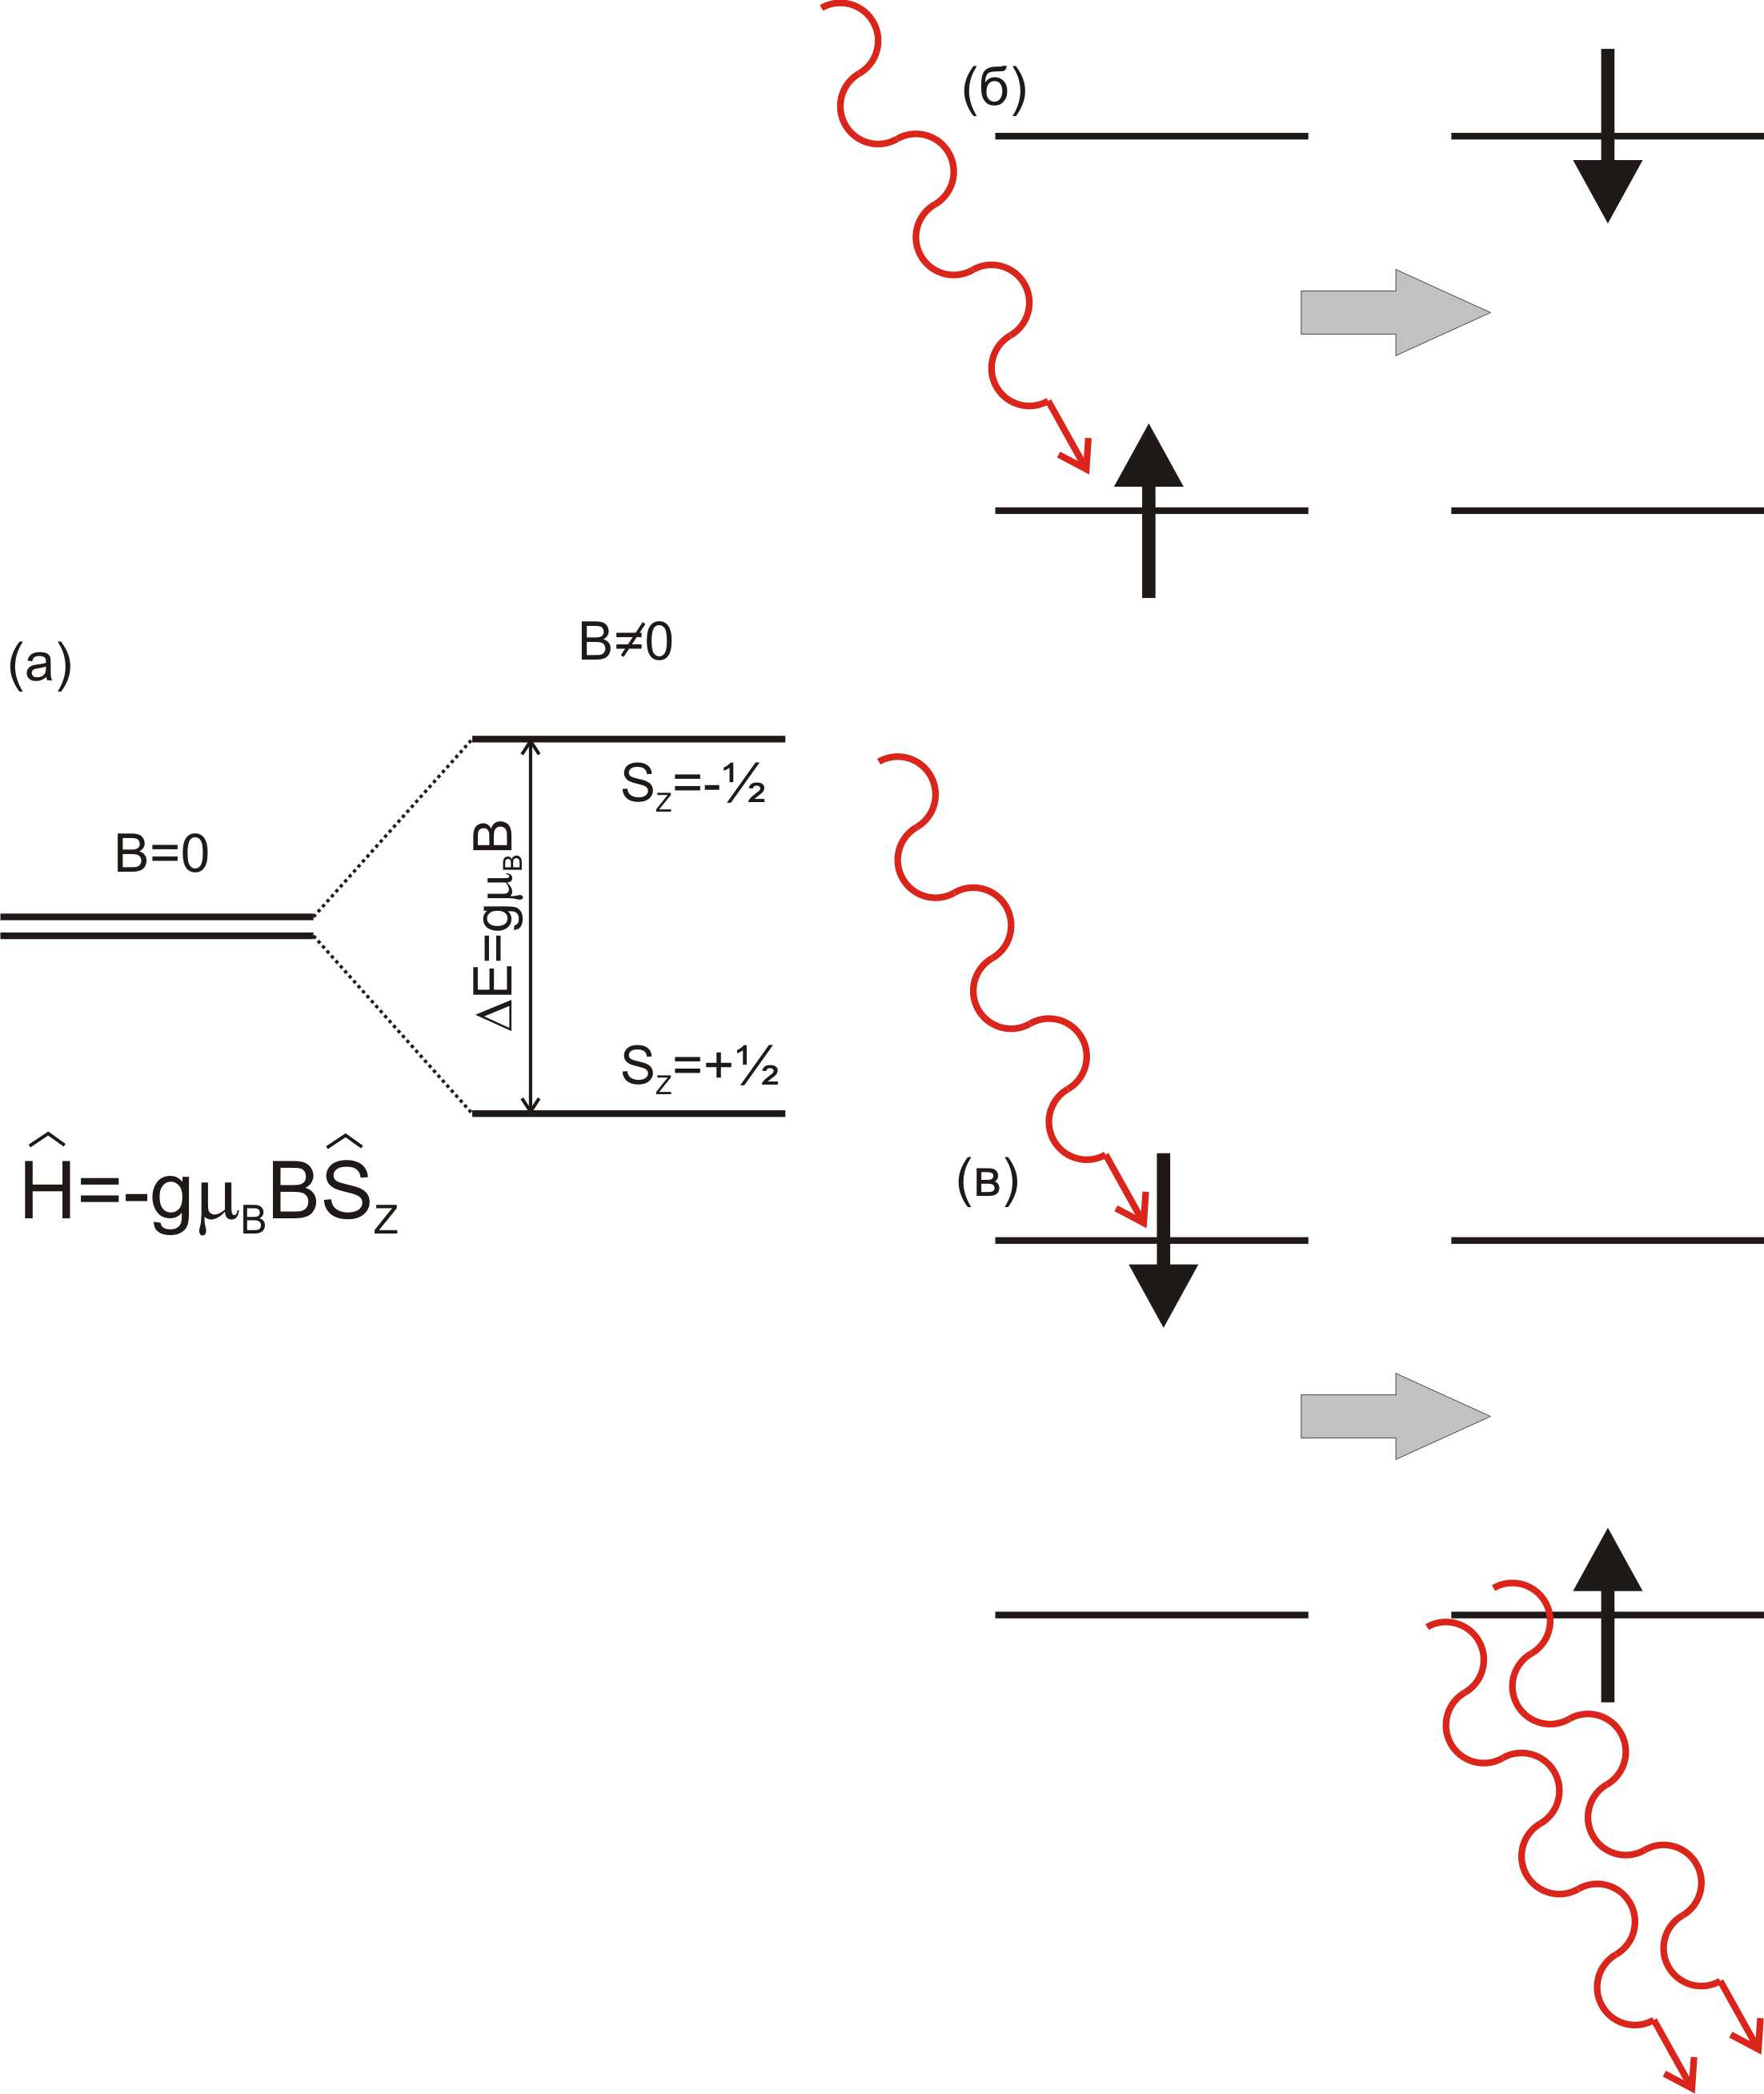
\includegraphics[width = 0.45\textwidth]{pics/schema-1.png}
        \caption{Схема резонансного поглощения электромагнитного излучения для изолированного спина $S=1/2$. (a) Зеемановское расщепление; (б) переход «снизу-вверх» с поглощением фотона $h\nu=g\mu_B B$; (в) переход «сверху-вниз» с излучением фотона}
    \label{pic:schema-1}
    \end{center}
\end{figure}
\FloatBarrier


Простейшей моделью является система из невзаимодействующих частиц со спином $S=1/2$, помещённая во внешнее магнитное поле. В отсутствии магнитного поля энергии состояний с $S_z=\pm 1/2$ совпадают. Из-за эффекта Зеемана энергии этих состояний различаются. При облучении системой с энергией кванта $h\nu=g\mu_B B$ возможны индуцированные переходы между подуровнями с поглощением или испусканием фотона. В лабораторной работе используется частота порядка \SI{100}{\mega\hertz}.


Для наблюдения поглощения необходимо резонансное совпадение частоты излучения с зеемановским расщеплением. Технически удобнее фиксировать частоту излучения и изменять магнитное поле, регистрируя поглощаемую мощность.


Поглощение описывается мнимой частью магнитной восприимчивости
\begin{equation}
P_{\text{погл}}=\tfrac{1}{2}\,\omega b^2\,\chi''(\omega,B),
\end{equation}
где $\omega$ --- частота переменного поля, $b$ --- амплитуда переменного поля, $B$ --- постоянное поле, $\chi''$ --- мнимая часть высокочастотной магнитной восприимчивости (в условиях работы различие между $\vb{B}$ и $\vb{H}$ пренебрежимо).


\subsection*{Физические причины возникновения резонансного поглощения в парамагнетике}
Парамагнетик - система слабо взаимодействующих магнитных диполей. Описание возможно в «классическом» подходе прецессии магнитного момента или в квантовомеханическом подходе переходов между зеемановскими подуровнями.


Классически уравнение прецессии:
\begin{equation}
\dv{\vb{M}}{t}=\gamma\,\vb{M}\times\vb{B}, \qquad \Omega_L=\gamma B.
\end{equation}
При совпадении частоты переменного поля с ларморовской $\Omega_L$ возникает резонанс.


Квантово расщепление терма описывается эффективным $g$-фактором $E(m)=g_{\text{эфф}}\mu_B B m$; для $S$-состояний и ряда радикалов $g_{\text{эфф}}\approx 2.0$. Частота М1-перехода: $h\nu=g_{\text{эфф}}\mu_B B$.

\section{Экспериментальная установка}

\FloatBarrier
\begin{figure}[h]
    \begin{center}
        
\includegraphics[width = 0.45\textwidth]{pics/ustan.png}
        \caption{Схема установки}
    \label{pic:ustan}
    \end{center}
\end{figure}
\FloatBarrier

Схема установки представлена на рис. \ref{pic:ustan}. Образец (порошок ДФПГ) в стеклянной ампуле помещается внутрь катушки индуктивности, входящей в состав колебательного контура. Входящий в состав контура конденсатор состоит из двух пластин, разделённых воздушным зазором, одна из пластин может перемещаться поворотом штока. Колебания в контуре возбуждаются антенной, соединённой с генератором высокой частоты (ВЧ) Г4-116. Амплитуда колебаний поля в катушке индуктивности
измеряется по наводимой в петле связи ЭДС индукции. Высокочастотные колебания ЭДС
индукции в приёмном контуре детектируются диодом, измеряемая при помощи
осциллографа низкочастотная огибающая этого сигнала пропорциональна квадрату
амплитуды колебаний поля в катушке.\\
Постоянное магнитное поле создаётся пропусканием тока от источника постоянного тока через основные катушки. При этом при помощи вольтметра измеряется падение напряжения на резисторе в цепи основных катушек. Переменное поле небольшой амплитуды создаётся подачей на модуляционные катушки напряжения с регулируемого трансформатора ЛАТР. Для измерения амплитуды колебаний переменного поля используется пробная катушка известной геометрии, подключённая к вольтметру. Пусть поток через неё $\Phi_{\text{проб}}$, тогда ЭДС индукции
\[\mathcal{E} = - \dfrac{d\Phi_{\text{проб}}}{dt}.\]
Если $I_{\text{осн}}$ -- ток через основную катушку, а $M$ -- взаимная индуктивность основной и пробной катушек, то
\[\Phi_{\text{проб}} = M I_{\text{осн}}.\]
Тогда амплитудное значение ЭДС индукции
\[\mathcal{E}_{\text{амп}} = - \dfrac{dM I_{\text{осн}}}{dt} = M \omega I_{\text{амп}}.\]
Учитывая, что $I_{\text{амп}} = \sqrt{2} I_{\text{действ}}=\frac{V_r}{r}$, где $V_R$, $R$ -- напряжение на резисторе с сопротивлением $R$ в цепи основных катушек, а также $\mathcal{E}_{\text{амп}} = \sqrt{2}\mathcal{E}_{\text{ср}}$, получим
\[\mathcal{E}_{\text{ср}} = M \omega \dfrac{V_R}{R} = k V_R.\]
Тогда, зная, что
\[\Phi_{\text{проб}} = B_0 N_{\text{проб}} \dfrac{\pi d_{\text{проб}}^2}{4} =  \dfrac{MU_R}{R} = \dfrac{k U}{\omega},\]
где $U$ -- напряжение на $R$ в резонансе, получим
\begin{equation}\label{1}
B_0 = \dfrac{4k U}{\pi \omega d^2_{\text{проб}} N_{\text{проб}}}.
\end{equation}
Характеристики катушек: пробная катушка $N_{\text{проб}} = 49$, $d_{\text{проб}} = 14.5\pm 0.1~\text{мм}$, основная катушка $N_{\text{осн}} = 5500$, $d_{\text{осн}} = 0.25\pm 0.01~\text{м}$,  модулирующая катушка $N_{\text{мод}} = 1500$, $d_{\text{мод}} = 0.30\pm 0.01~\text{м}$.

\section{Результаты измерений и обработка данных}

\subsection*{Настройка ВЧ генератора}

Сначала настроим ВЧ-генератор на резонансную частоту колебательного контура. По показаниям частотомера (или шкалы генератора) получаем частоту
\[
    f_0 \approx 161{.}710~\text{МГц}.
\]
Далее устанавливаем добротную настройку контура по максимуму амплитуды сигнала в тракте детектирования. При отклонении частоты от $f_0$ амплитуда заметно уменьшается, что соответствует узкой полосе пропускания контура.

\subsection*{Наблюдение сигнала резонансного поглощения}

Переведём осциллограф в режим временной развёртки и подадим в модуляционные катушки переменное магнитное поле. На экране наблюдается сигнал резонансного поглощения в образце ДФПГ. При грубой настройке постоянного поля линия смещена относительно центра развертки.

При более точной настройке постоянного поля на резонанс пики сигнала следуют с удвоенной частотой модулиции, что соответствует двукратному прохождению поля через резонанс за период модуляционного сигнала.

При увеличении амплитуды переменного поля фиксируется рост амплитуды резонансных пиков и последующее их раздвоение при превышении амплитудой модулирующего поля характерной ширины линии.

\FloatBarrier

\subsection*{Точная настройка резонансного поля и определение ширины линии}

Далее переведём осциллограф в режим XY-развёртки и выполним точную настройку постоянного поля на центр линии ЭПР. В этом режиме наблюдается симметричная линия поглощения.

Амплитуда модулирующего поля $B_{\text{мод}}$ определяется по ЭДС $\varepsilon_i$ в пробной катушке известной геометрии при подаче в основные катушки переменного тока.
\[
    B_{\text{мод}} 
    = \sqrt{2}\,\cfrac{2 \varepsilon_i}{\pi^2 d^2 N_\text{проб} \nu}
    = \sqrt{2}\,\cfrac{2 \cdot 7{.}70\cdot10^{-3}\,\text{В}}
        {\pi^2 \,(14{.}9\cdot10^{-3}\,\text{м})^2 \cdot 44 \cdot 50\,\text{Гц}}
    \approx 4{.}52~\text{мТл}.
\]

Погрешность $B_{\text{мод}}$ оценим через частные производные, погрешности величин берем как половину последнего известного разряда:

\begin{multline*}
    \sigma_{B_{\text{мод}}} = 
    \sqrt{
        \left( \cfrac{\partial B_{\text{мод}}}{\partial \varepsilon_i} \right)^2 \sigma_{\varepsilon_i}^2 +
        \left( \cfrac{\partial B_{\text{мод}}}{\partial d} \right)^2 \sigma_{d}^2 +
        \left( \cfrac{\partial B_{\text{мод}}}{\partial \nu} \right)^2 \sigma_{\nu}^2 } = \\
        = \sqrt{
        \left( \frac{B_{\text{мод}}}{\varepsilon_i} \right)^2 \sigma_{\varepsilon_i}^2 +
        \left( -2\,\frac{B_{\text{мод}}}{d} \right)^2 \sigma_{d}^2 +
        \left( -\,\frac{B_{\text{мод}}}{\nu} \right)^2 \sigma_{\nu}^2 } = \\ 
        = B_{\text{мод}} \sqrt{
        \left( \frac{\sigma_{\varepsilon_i}}{\varepsilon_i} \right)^2 +
        \left( 2\,\frac{\sigma_{d}}{d} \right)^2 +
        \left( \frac{\sigma_{\nu}}{\nu} \right)^2 }
\end{multline*}

Тогда получаем 

\[B_{\text{мод}} = (4{.}52 \pm 0{.}6)~\text{мТл}\]


С осциллограммы в режиме XY измеряем полную высоту линии 
$A_{\text{полн}} = 29$ и высоту на половине максимума 
$A_{1/2} = 2{.}5$. Тогда полуширина линии в единицах поля определяется соотношением
\[
    \Delta B = \frac{A_{1/2}}{A_{\text{полн}}} B_{\text{мод}}
             = \frac{2{.}5}{29}\cdot 4{.}52~\text{мТл}
             \approx 0{.}39~\text{мТл},
\]

Погрешность $\sigma_{\Delta B}$ оценим как:

\begin{equation*}
    \sigma_{\Delta B} 
    = \Delta B \sqrt{
        \left( \frac{\sigma_{A_{1/2}}}{A_{1/2}} \right)^2 +
        \left( \frac{\sigma_{A_{\text{полн}}}}{A_{\text{полн}}} \right)^2 +
        \left( \frac{\sigma_{B_{\text{мод}}}}{B_{\text{мод}}} \right)^2 }
\end{equation*}

Тогда 

\[
    \Delta B = (0{.}39 \pm 0{.}06)~\text{мТл}.
\]

\FloatBarrier

\subsection*{Калибровка поля электромагнита и определение g-фактора}

Для калибровки зависимости магнитного поля в зазоре электромагнита от тока в основных катушках подаём в них переменный ток от ЛАТРа. Измеряем ЭДС в цепи измерительной катушки и посчитаем поле в ней: $B = (5{.}7 \pm 0{.}1)~\text{мТл}$. Посчитаем g-фактор.

\[
    g= \cfrac{h f_0}{\mu_b B_0} \approx 2.033
\]

Погрешность вычислим:

\[
    \sigma_g = g\sqrt{\left( \cfrac{\sigma_{f_0}}{f_0} \right)^2 + \left( \cfrac{\sigma_{B}}{B} \right)^2}
\]

Тогда
\[
    g= (2{.}03 \pm 0{.}04)
\]

\subsection*{Ихмерение g-фактора при других резонансных частотах контура}

Используя винт внизу установки, поменяем расстояние между обкладками конденсатора так, чтобы частота увеличилась:

\[
    f \sim \frac{1}{C} \sim d 
\]

Новая частота $f_1 = 178{.}49~\text{МГц}$. Проведем для нее аналогичные измерения g-фактора

\[
    g= (2{.}02 \pm 0{.}03)
\]

Теперь измерим g-фактор для частоты ниже изначальной: $f_2 = 152.066~\text{МГц}$

\[
    g= (1{.}96 \pm 0{.}04)
\]

\subsection*{Определение добротности контура}

Измерим резонансную частоту: $f_0 = 153{.}060~\text{МГц}$. 

Добротность колебательного контура может быть определена по расстройке частоты до достижения сигналом половины от максимального значения

\[
    Q_0 = \frac{f_0}{f_{+ \frac{1}{2}} - f_{- \frac{1}{2}}} = \frac{153{.}060}{153{.}660 - 152{.}450} \approx 120
\]


\FloatBarrier
\end{document}